\section{Theorie}
\label{sec:Theorie}
Periodische Funktionen wiederholen sich nach bestimmten Zeit- bzw. Raumabständen
 $T$ und $D$.
Für diese gilt
\begin{align}
  f(x,t)=&f(x+D,t)\\
  f(x,t)=&f(x,t+T)\;\;.
\end{align}
Die beiden wichtigsten Beispiele dafür sind
\begin{align}
f(x,t)=A\sin\left(\frac{2\pi}{T}t+\frac{2\pi}{D}x\right) \\
f(x,t)=A\cos\left(\frac{2\pi}{T}t+\frac{2\pi}{D}x\right)
\end{align}
Diese Funktionen lassen sich mit der Fourier-Reihe approximieren dafür verwendet
mand das Fourier-Theorem
\subsection{Fouriersche Theorem}
Das Fourier Theorem besagt, dass die Reihe
\begin{equation}
f(t)=\frac{1}{2}a_0+\sum_{n=0}^\infty\left(a_n \cos\left(\frac{2n\pi}{T}t\right)
+b_n\sin\left(\frac{2n\pi}{T}t\right)\right)
\label{fuireihe}
\end{equation}
eine periodische Funktion beschreibt, wenn die Reihe konvergiert und für die
Koeffizienten $a_n$ und $b_n$
\begin{equation}
  a_n=\frac{2}{T}\int_a^b\,\,f(t)\cos\left(\frac{2n\pi}{T}t\right)
  \label{fuikoeffizient_a}
\end{equation}
\begin{equation}
  b_n=\frac{2}{T}\int_a^b\,\,f(t)\sin\left(\frac{2n\pi}{T}t\right)
  \label{fuikoeffizient_b}
\end{equation}
gilt. In der Fourier Entwicklung treten die Frequenz $\nu=\frac{1}{T}$, sowie
ihre ganzzahligen Vielfachen auf. Bei geraden Funktionen fallen alle $b_n$ weg,
da gilt $f(t)=f(-t)$ und dies bei sinus Funktionen nicht gegeben ist. Bei
ungeraden Funktionen fallen alle $a_n$ weg, da $f(t)=-f(-t)$ gilt und ein Kosinus
diese Bedingung nicht erfüllt. $a_n$ und $b_n$ müssen nach Gleichung
\eqref{fuireihe} für $\lim\limits_{n \to \infty}$ gegen Null gehen, damit die
Reihe konvergiert. Ein Beispiel dafür ist in Abbildung \ref{fig:Fouriertrafo}
dargestellt. Wenn $f(t)$ stetig ist folgt die Gleichmäßige Konvergenz. Ist $f(t)$
unstetig, so lässt sie sich an dieser Stelle nicht mit der Fourier-Reihe
approximieren. Es tritt das Gibbsche Phänomen auf, das die Abweichung beschreibt.
\begin{figure}
  \centering
  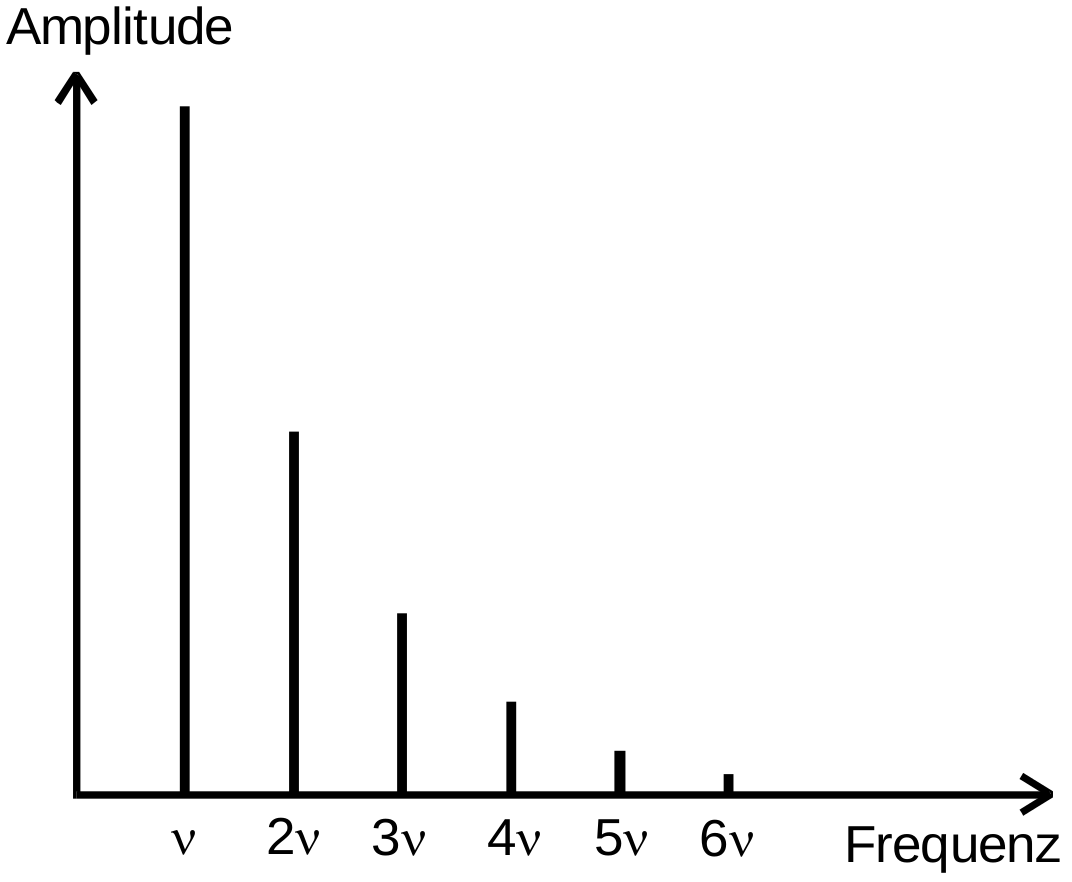
\includegraphics[width=0.4\textwidth]{Fouriertrafo.png}
  \caption{Fouriertransformation \cite{sample}.}
  \label{fig:Fouriertrafo}
\end{figure}
\subsection{Fourier-Transformation}
\label{sec:Fourier-Transformation}
Mit der Fourier-Transformation lässt sich das gesamte Frequenzspektrum einer
zeitabhängigen Funktion bestimmen. Die Fourier-Transformation ist definiert durch:
\begin{equation}
  g(\nu)= \int_{-\infty}^\infty f(t)\exp(i\nu t) \mathrm{d}t
\end{equation}
Sollte $f(t)$ periodisch sein, ist $g(\nu)$ eine konvergierende Reihe von
$\delta$-Funktionen wie die in Abbildung \ref{fig:Fouriertrafo}. Die Umkehrfunktion
\begin{equation}
  f(t)= \frac{1}{2\pi}\int_{-\infty}^\infty g(\nu)\exp(i\nu t) \mathrm{d}\nu
\end{equation}
ergibt aus dem Frequenzspektrum $g(\nu)$ wieder die Funktion $f(t)$. In der
Praxis ist eine genaue Fourier-Transformation nicht möglich, da über einen unendlichen
Zeitraum integriert werden muss. Mit endlichen Integrationsgenzen ist keine
Periodizität mehr gegeben, dadurch ergibt sich aus der Transformation keine Reihe
von $\delta$-Funktionen sondern überall stetige Funktionen. Zudem entstehen
Nebenmaxima zu den ursprünglichen Hauptmaxima.
\subsection{Fourier-Analyse}
\label{sec:Fourier-Analyse}
Mit der Fourier-Analyse, werden Signale in Fourier-Koeffizienten aufgeteilt, mit
denen durch die Gleichungen \eqref{fuireihe}, \eqref{fuikoeffizient_a}
und \eqref{fuikoeffizient_b} die analysierten Schwingungen approximiert werden können.
\subsection{Lissajous-Figuren}
Lissajous-Figuren entstehen, durch die Überlagerung von zwei harmonischen
Funktionen die senkrecht zueinander stehen. Mit diesen lässt sich die Phasendifferenz
zwischen zwei Oberwellen bestimmen.
Die Phasendifferenz ist $0$ bei einem Frequenzverhältnis von $1:2$, wenn es sich um
eine geschlossende Kurve handelt die einen Schnitt in der mitte hat.
Bei einem Frequenzverhältnis von $1:3$, ist die Phasendifferenz $0$ wenn es sich
um eine offene Kurve handelt deren enden links oben und rechts unten sind.
\subsection{Abtasttheorem}
Das Abstasttheorem
\begin{equation}
  \nu_A\l2\nu_{max}
\end{equation}
Besagt, dass der Fehler bei der Fourier-Transformation vernachlässigbar klein wird,
wenn die Abstastfrequenz $\nu_A$ größer ist, als das doppelte der höchsten Frequenz
des analysierten Signals.
\cite{sample}
